\section{Seasonal forecasting of the polar stratosphere and its coupling
with the
troposphere}\label{seasonal-forecasting-of-the-polar-stratosphere-and-its-coupling-with-the-troposphere}

\subsection{Figures and captions}\label{figures-and-captions}

\begin{figure}[htbp]
\centering
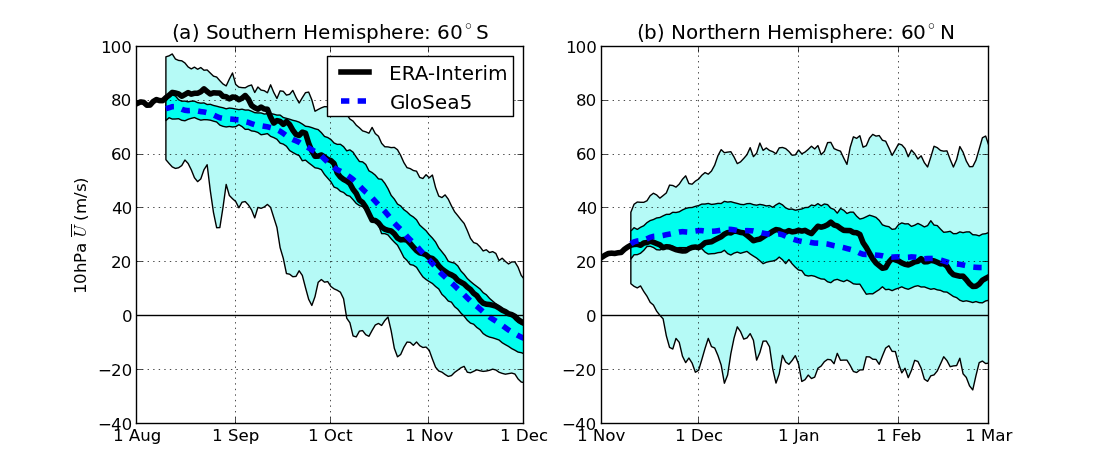
\includegraphics{./figures/zm_winds.png}
\caption{Time series of 10 hPa zonal-zonal mean zonal wind
($\overline{U}$) at 60$^{\circ}$S for GloSea5 hindcasts initialised near
1st August (a) and at 60$^{\circ}$N for hindcasts initialised near 1st
November (b). The ERA-Interim mean over 1996-2009 (black line) and the
GloSea5 mean over all ensemble members (blue dashed line) are shown,
along with the interquartile range and range of all ensemble members.}
\end{figure}

\begin{figure}[htbp]
\centering
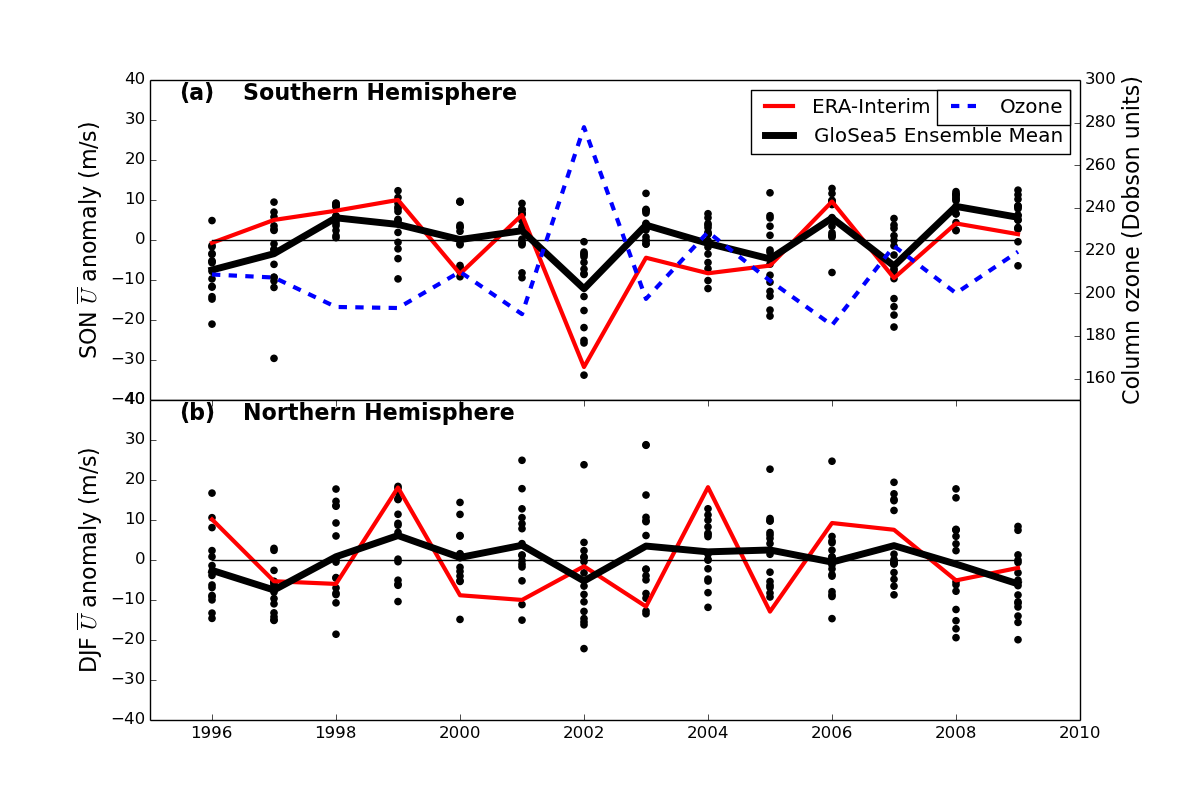
\includegraphics{./figures/seas_winds.png}
\caption{Time series of stratospheric polar vortex (60$^{\circ}$S/N,
10hPa) zonal-mean zonal wind anomalies, averaged over SON for the
Southern Hemisphere (a) and DJF for the Northern Hemisphere (b). Dots
indicate individual GloSea5 ensemble members, the thick black line the
ensemble mean, and the thin red line ERA-Interim. The correlation of the
GloSea5 ensemble mean and ERA-Interim is 0.74 in the SH and 0.16 in the
NH. Also plotted in (a) is the polar cap (60-90$^{\circ}$S) SON mean
total column ozone from ERA-Interim (blue dashed line).}
\end{figure}

\begin{figure}[htbp]
\centering
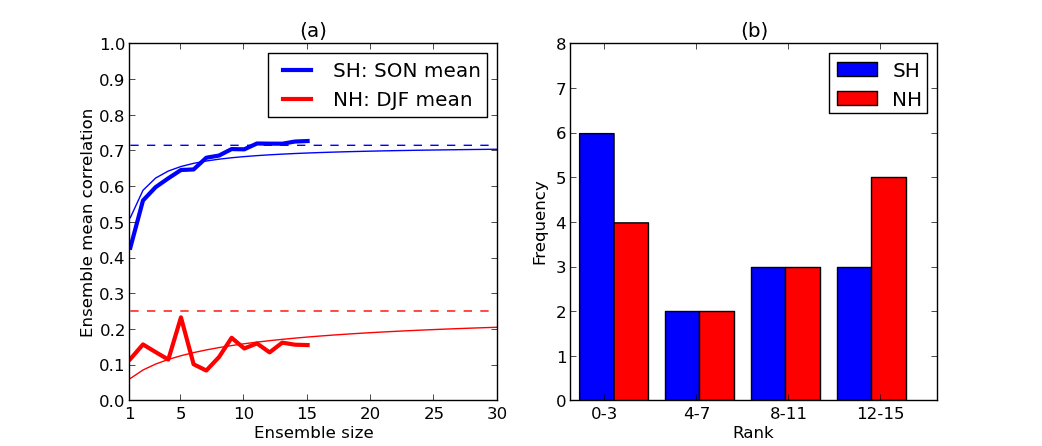
\includegraphics{./figures/ens_hist.png}
\caption{(a) Variation with ensemble size (between 1-15) of GloSea
ensemble mean correlation with ERA-Interim for stratospheric polar
vortex $\overline{U}$ anomalies (thick lines), with a fitted theoretical
distribution {[}Sardeshmukh et al., 2000{]} (thin lines) and its
asymptote (dashed line). (b) Rank histogram of vortex wind anomalies,
showing where observed values lie in the ensemble hindcasts.}
\end{figure}

\begin{figure}[htbp]
\centering
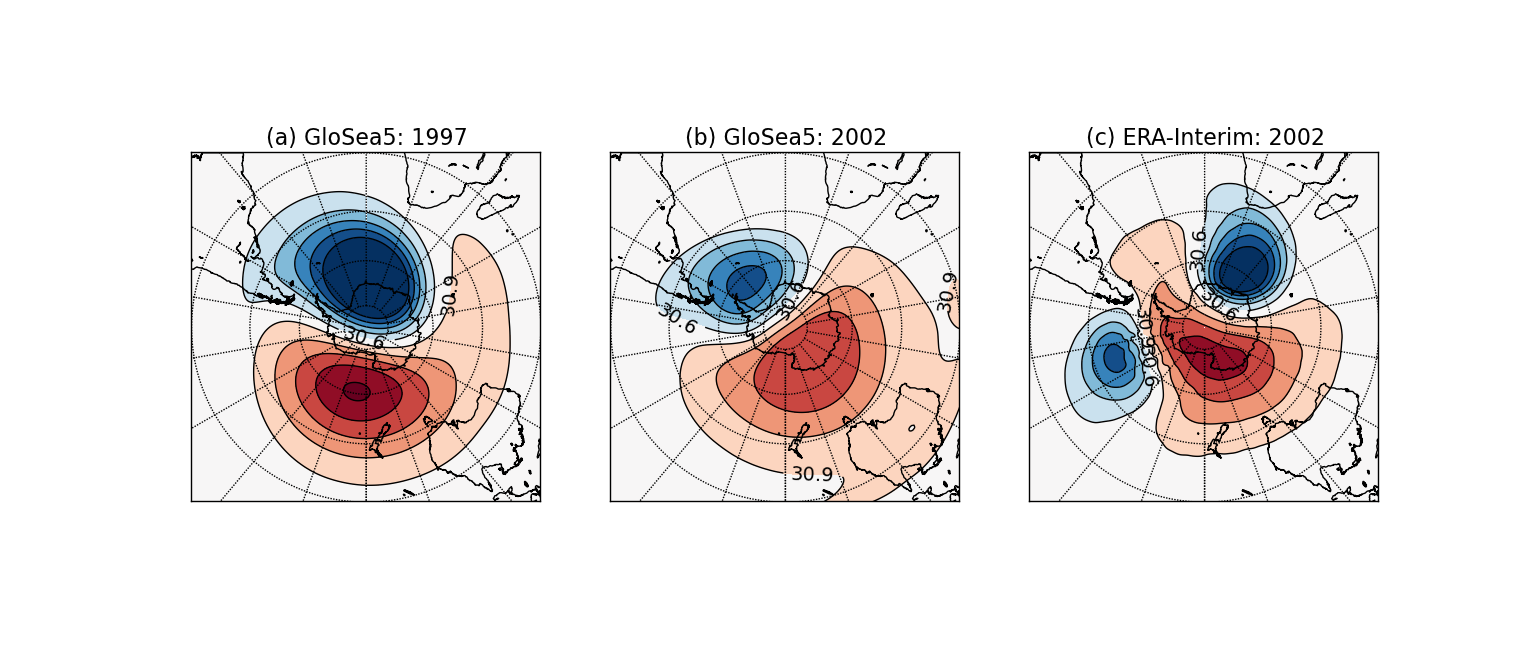
\includegraphics{./figures/sh_ssws.png}
\caption{Geopotential height at 10hPa at the central date (date at which
Uat 60$^{\circ}$S, 10 hPa is at its minimum value) of the two GloSea5
ensemble members which simulate a SH SSW (a,b), and for ERA-Interim at
the central date of the 2002 SSW (c). Units are km and the contour
interval is 0.3 km.}
\end{figure}

\begin{figure}[htbp]
\centering
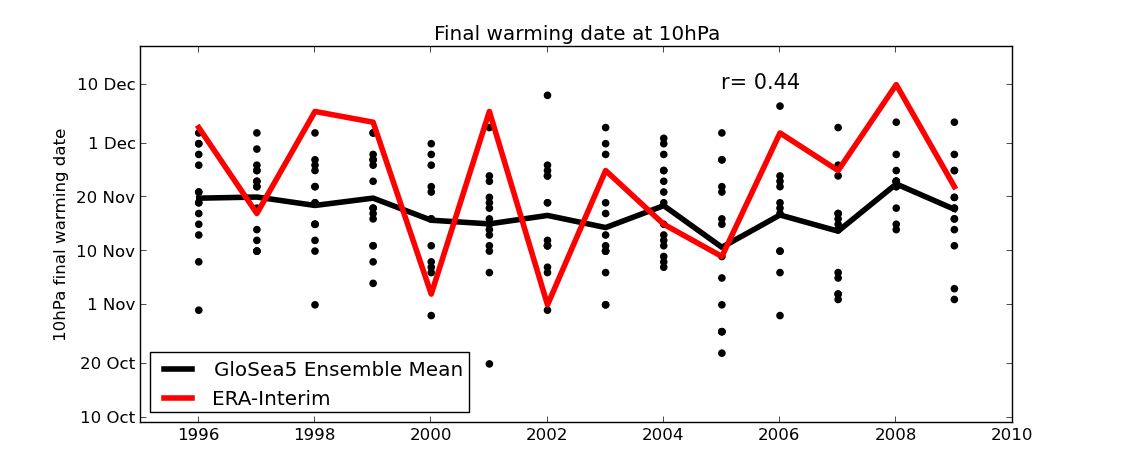
\includegraphics{./figures/glosea_fw.png}
\caption{Time series of the SH final warming date at 10hPa in GloSea5
and ERA-Interim. The final warming date is defined as the date at which
Uat 60$^{\circ}$S, 10hPa becomes negative for the last time. The
correlation between the GloSea5 ensemble mean and ERA-Interim is 0.44
which is statistically significant at the 95\% level.}
\end{figure}

\begin{figure}[htbp]
\centering
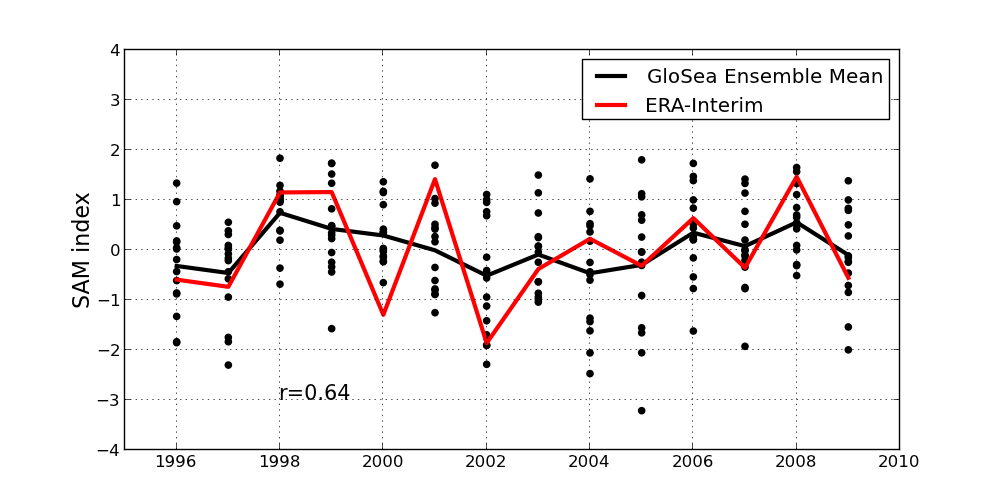
\includegraphics{./figures/sam.png}
\caption{SON mean Southern Annular Mode (SAM) index in individual
GloSea5 ensemble members (dots), ensemble mean (black line) and
ERA-Interim. The SAM is calculated from mean sea-level pressure data.
The correlation of the ensemble mean and ERA-Interim values is 0.64,
which is statistically significant at the 99\% level.}
\end{figure}

\begin{figure}[htbp]
\centering
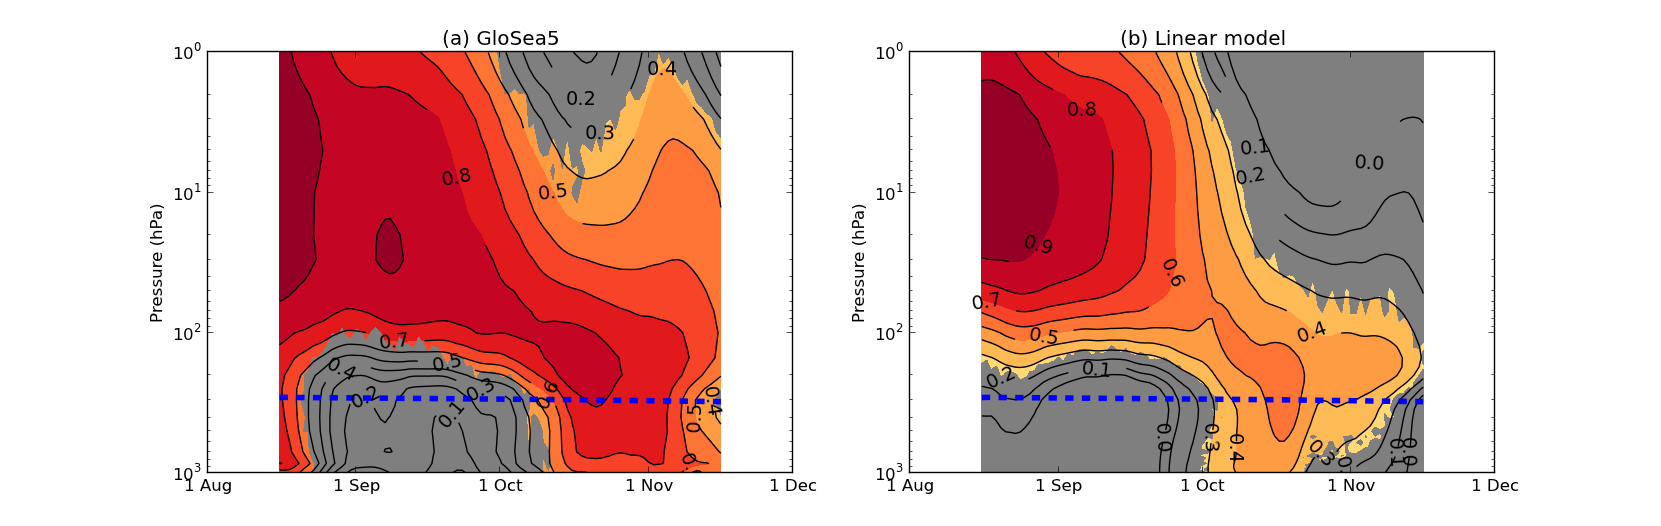
\includegraphics{./figures/glosea_linear_corr.png}
\caption{(a) Correlation of GloSea5 ensemble mean polar cap
(60-90$^{\circ}$S) geopotential height anomalies ($Z'$) with ERA-Interim
values, as a function of time and height for forecasts initialised near
1st August. (b) Correlation of ERA-Interim $Z'$ values with those
predicted by the linear statistical model based on $Z'$ at 10 hPa on
15th August. $Z'$ values are smoothed using a 30 moving window. Grey
shading indicates regions which not are greater than zero at the 95\%
confidence interval. The blue dashed line indicates the polar cap mean
tropopause level from Wilcox et al., 2012.}
\end{figure}

\begin{figure}[htbp]
\centering
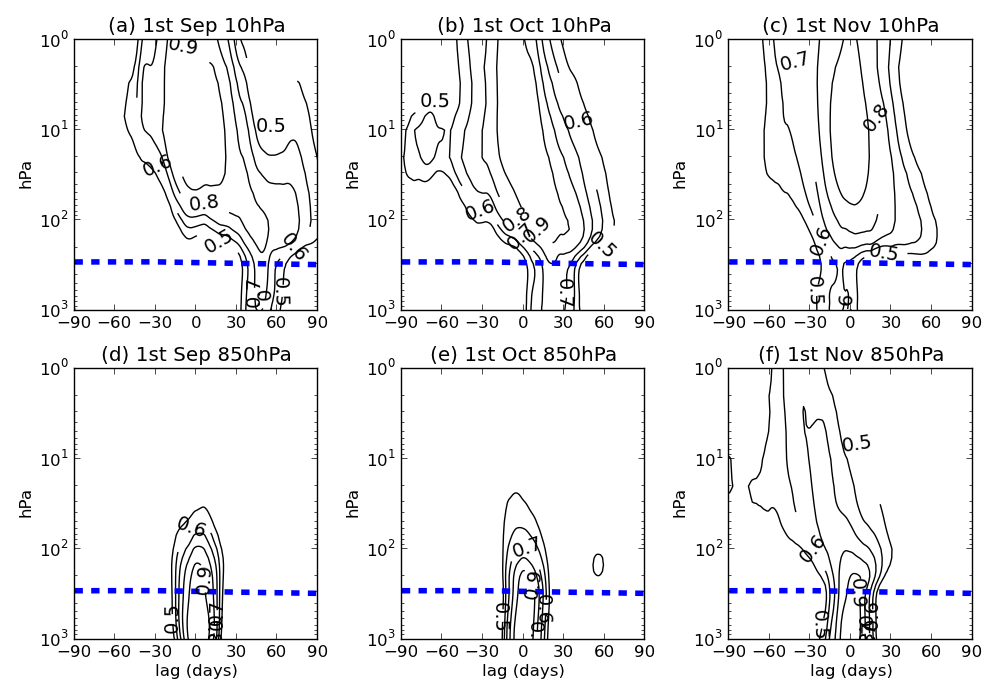
\includegraphics{./figures/lag_corrs_SH_10hPa.png}
\caption{Lag-height correlations of SH polar cap (60-90$^{\circ}$S)
geopotential height anomalies (Z') in ERA-Interim. $Z'$ values are
smoothed with a 30-day running mean before calculating correlations.
(a,b,c) Show correlations with $Z'$ at 10 hPa on the 1st of September,
October and November respectively. (d,e,f) Show correlations with $Z'$
at 850 hPa. The blue dashed line indicates the polar cap mean tropopause
level from Wilcox et al., 2012. ADD SIGNIFICANCE TESTS}
\end{figure}

\begin{figure}[htbp]
\centering
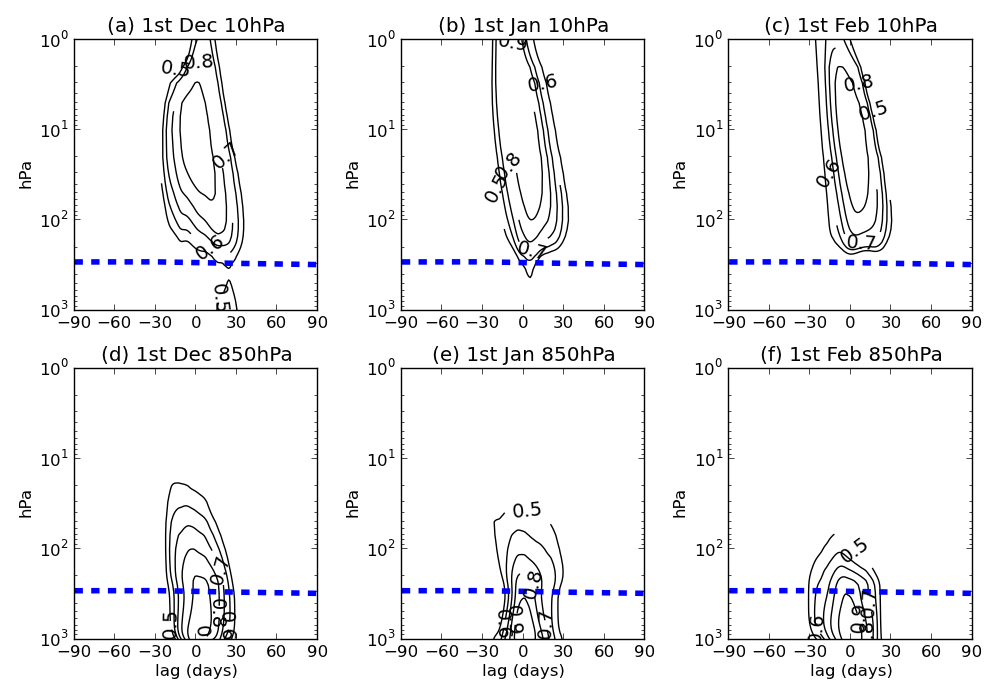
\includegraphics{./figures/lag_corrs_NH_DJF.png}
\caption{As Figure 8 but for the NH polar cap (60-90$^{\circ}$N), with
correlations calculated from 1st December, January and February
respectively. ADD SIGNIFICANCE TESTS \label{figure}}
\end{figure}

This is a reference \ref{figure}
